
During the dedicated experiment that took place in the SPS
in 2018 with the CCs, the measured emittance
growth was found to be a factor four (on average) lower than
expected from the theory (see Section~\ref{sec:meas_2018_vs_theory}). The reason for this discrepancy remained unresolved for some time, as detailed follow-up studies (see Chapter~\ref{Ch:investigating_discrepancy}) investigated and excluded a number of possible explanations for the discrepancy.
It was recently found, that the beam transverse impedance, which is not included in the theory~\cite{PhysRevSTAB.18.101001} used for the comparison with the measurements may impact the noise-induced emittance growth and explain the experimental observations. Here, the damping mechanism from the beam transverse impedance is investigated as observed in detailed PyHEADTAIL simulations.

The structure of this chapter is as follows:




\section{SPS transverse impedance model}\label{sec:sps_impedance_model}
The PyHEADTAIL studies presented in this chapter are performed including the detailed transverse impedance model of the SPS machine~\cite{sps_impedance_model_git}. This model has been developed through a combination of theoretical computations, electromagentic simulations and was benchmarked with beam-based measurements~\cite{Salvant:1274254, Zannini:1561199, Salvant:1271349, Zannini:2141779}. 
It includes the contributions from all the individual elements in the SPS lattice i.e. the resistive wall, the indirect space charge, the kickers, the RF cavities (200\,MHz and 800\,MHz), the step transitions and the horizontal and vertical beam position monitors~\cite{Zannini:2141779}. As discussed in  Section~\ref{subsec:pyheadtail}, the model needs to represent the global impedance of the full machine. Thus, the total impedance is obtained by summing up the impedance of each element weighted with the beta function at its location and by dividing the sum by the average beta function of the SPS. For the Q26 optics the average horizontal and vertical beta functions are 42.09\,m and 42.01\,m respectively.
%https://indico.cern.ch/event/299470/contributions/686509/attachments/564150/777102/LIUSPS_transverse_imp_5.pdf
% The Wall contribution included both the resistive wall and the indirect SC.
Figure~\ref{fig:sps_impedance_model_H_V} shows the complete transverse impedance model of the SPS machine with the disentangled dipolar (blue) and quadrupolar (orange) terms to be plotted seperetaly. 

% Plot figures: /eos/user/n/natriant/Project_thesis/plot_wakefields_impedances_SPS
\begin{figure}[!ht]
    \centering
    \begin{subfigure}[t]{0.45\textwidth}
        \centering
        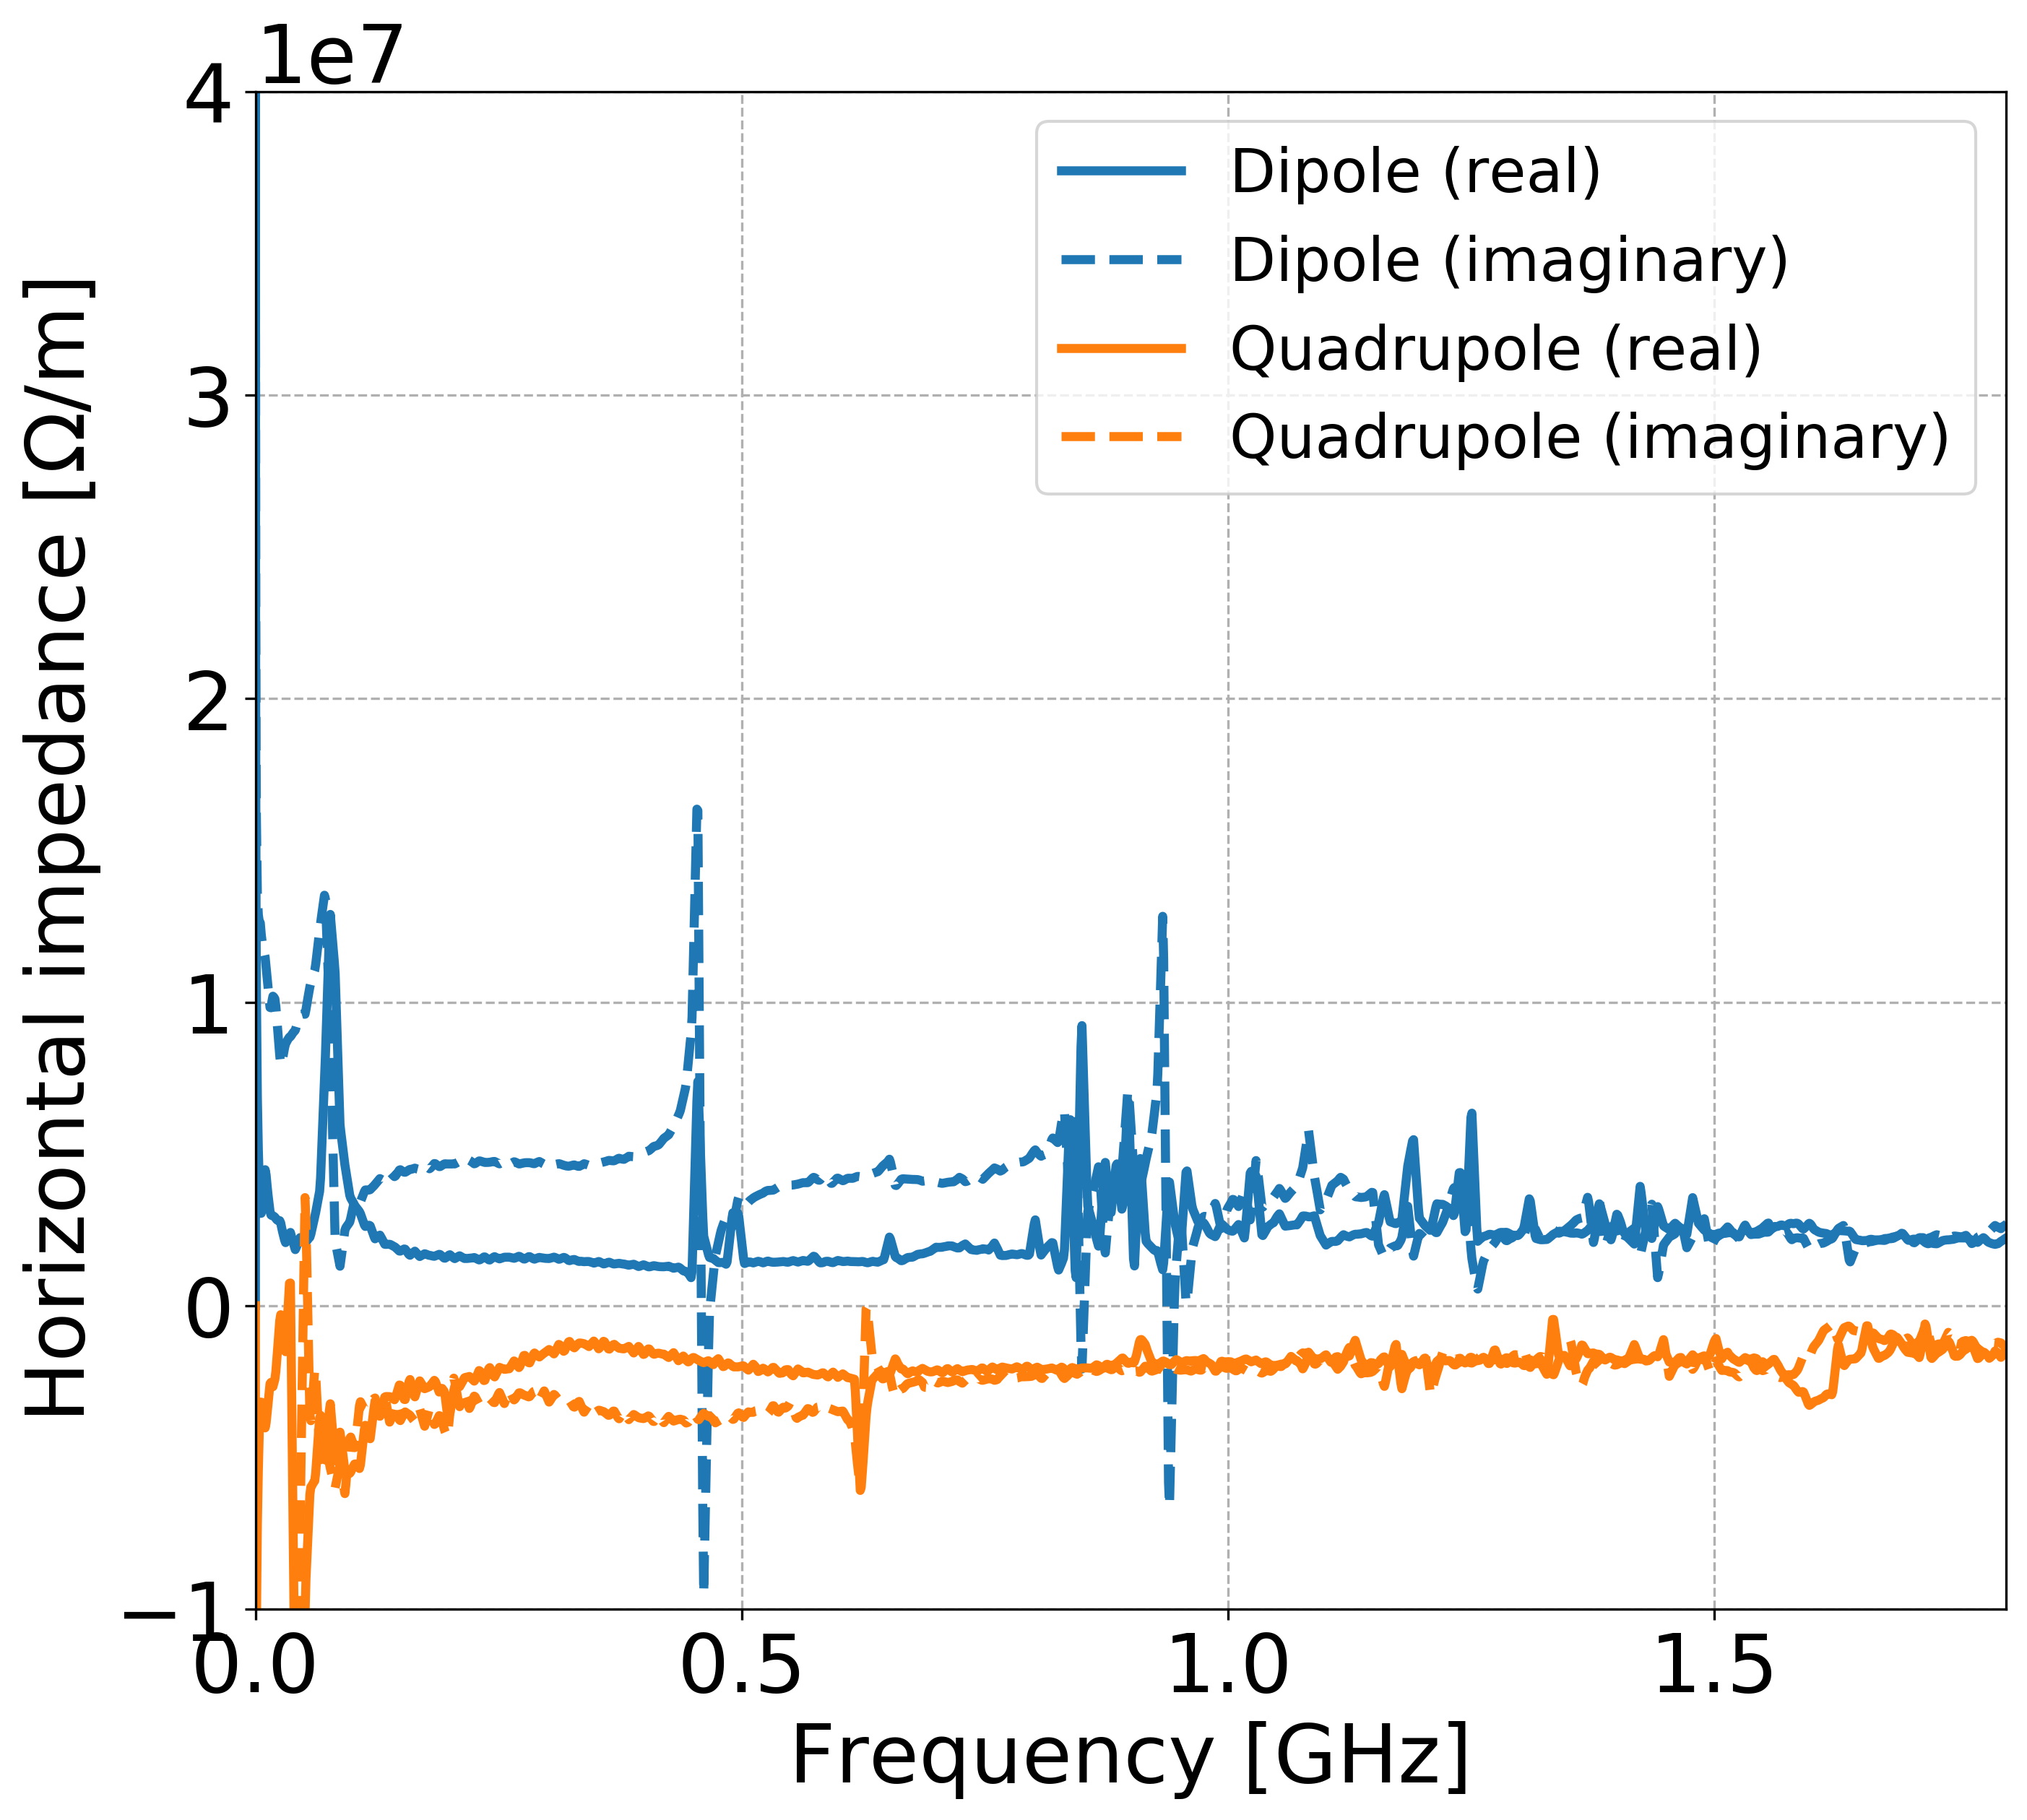
\includegraphics[width=1\textwidth]{images/Ch7/Q26_complete_SPS_model_impedance_H_plane.png}
        %\caption{$y=\sin(2 \pi f t),\ f=50$ Hz}
        %\label{fig:add_label_here}
    \end{subfigure}
    \hfill
    \begin{subfigure}[t]{0.45\textwidth}
        \centering
        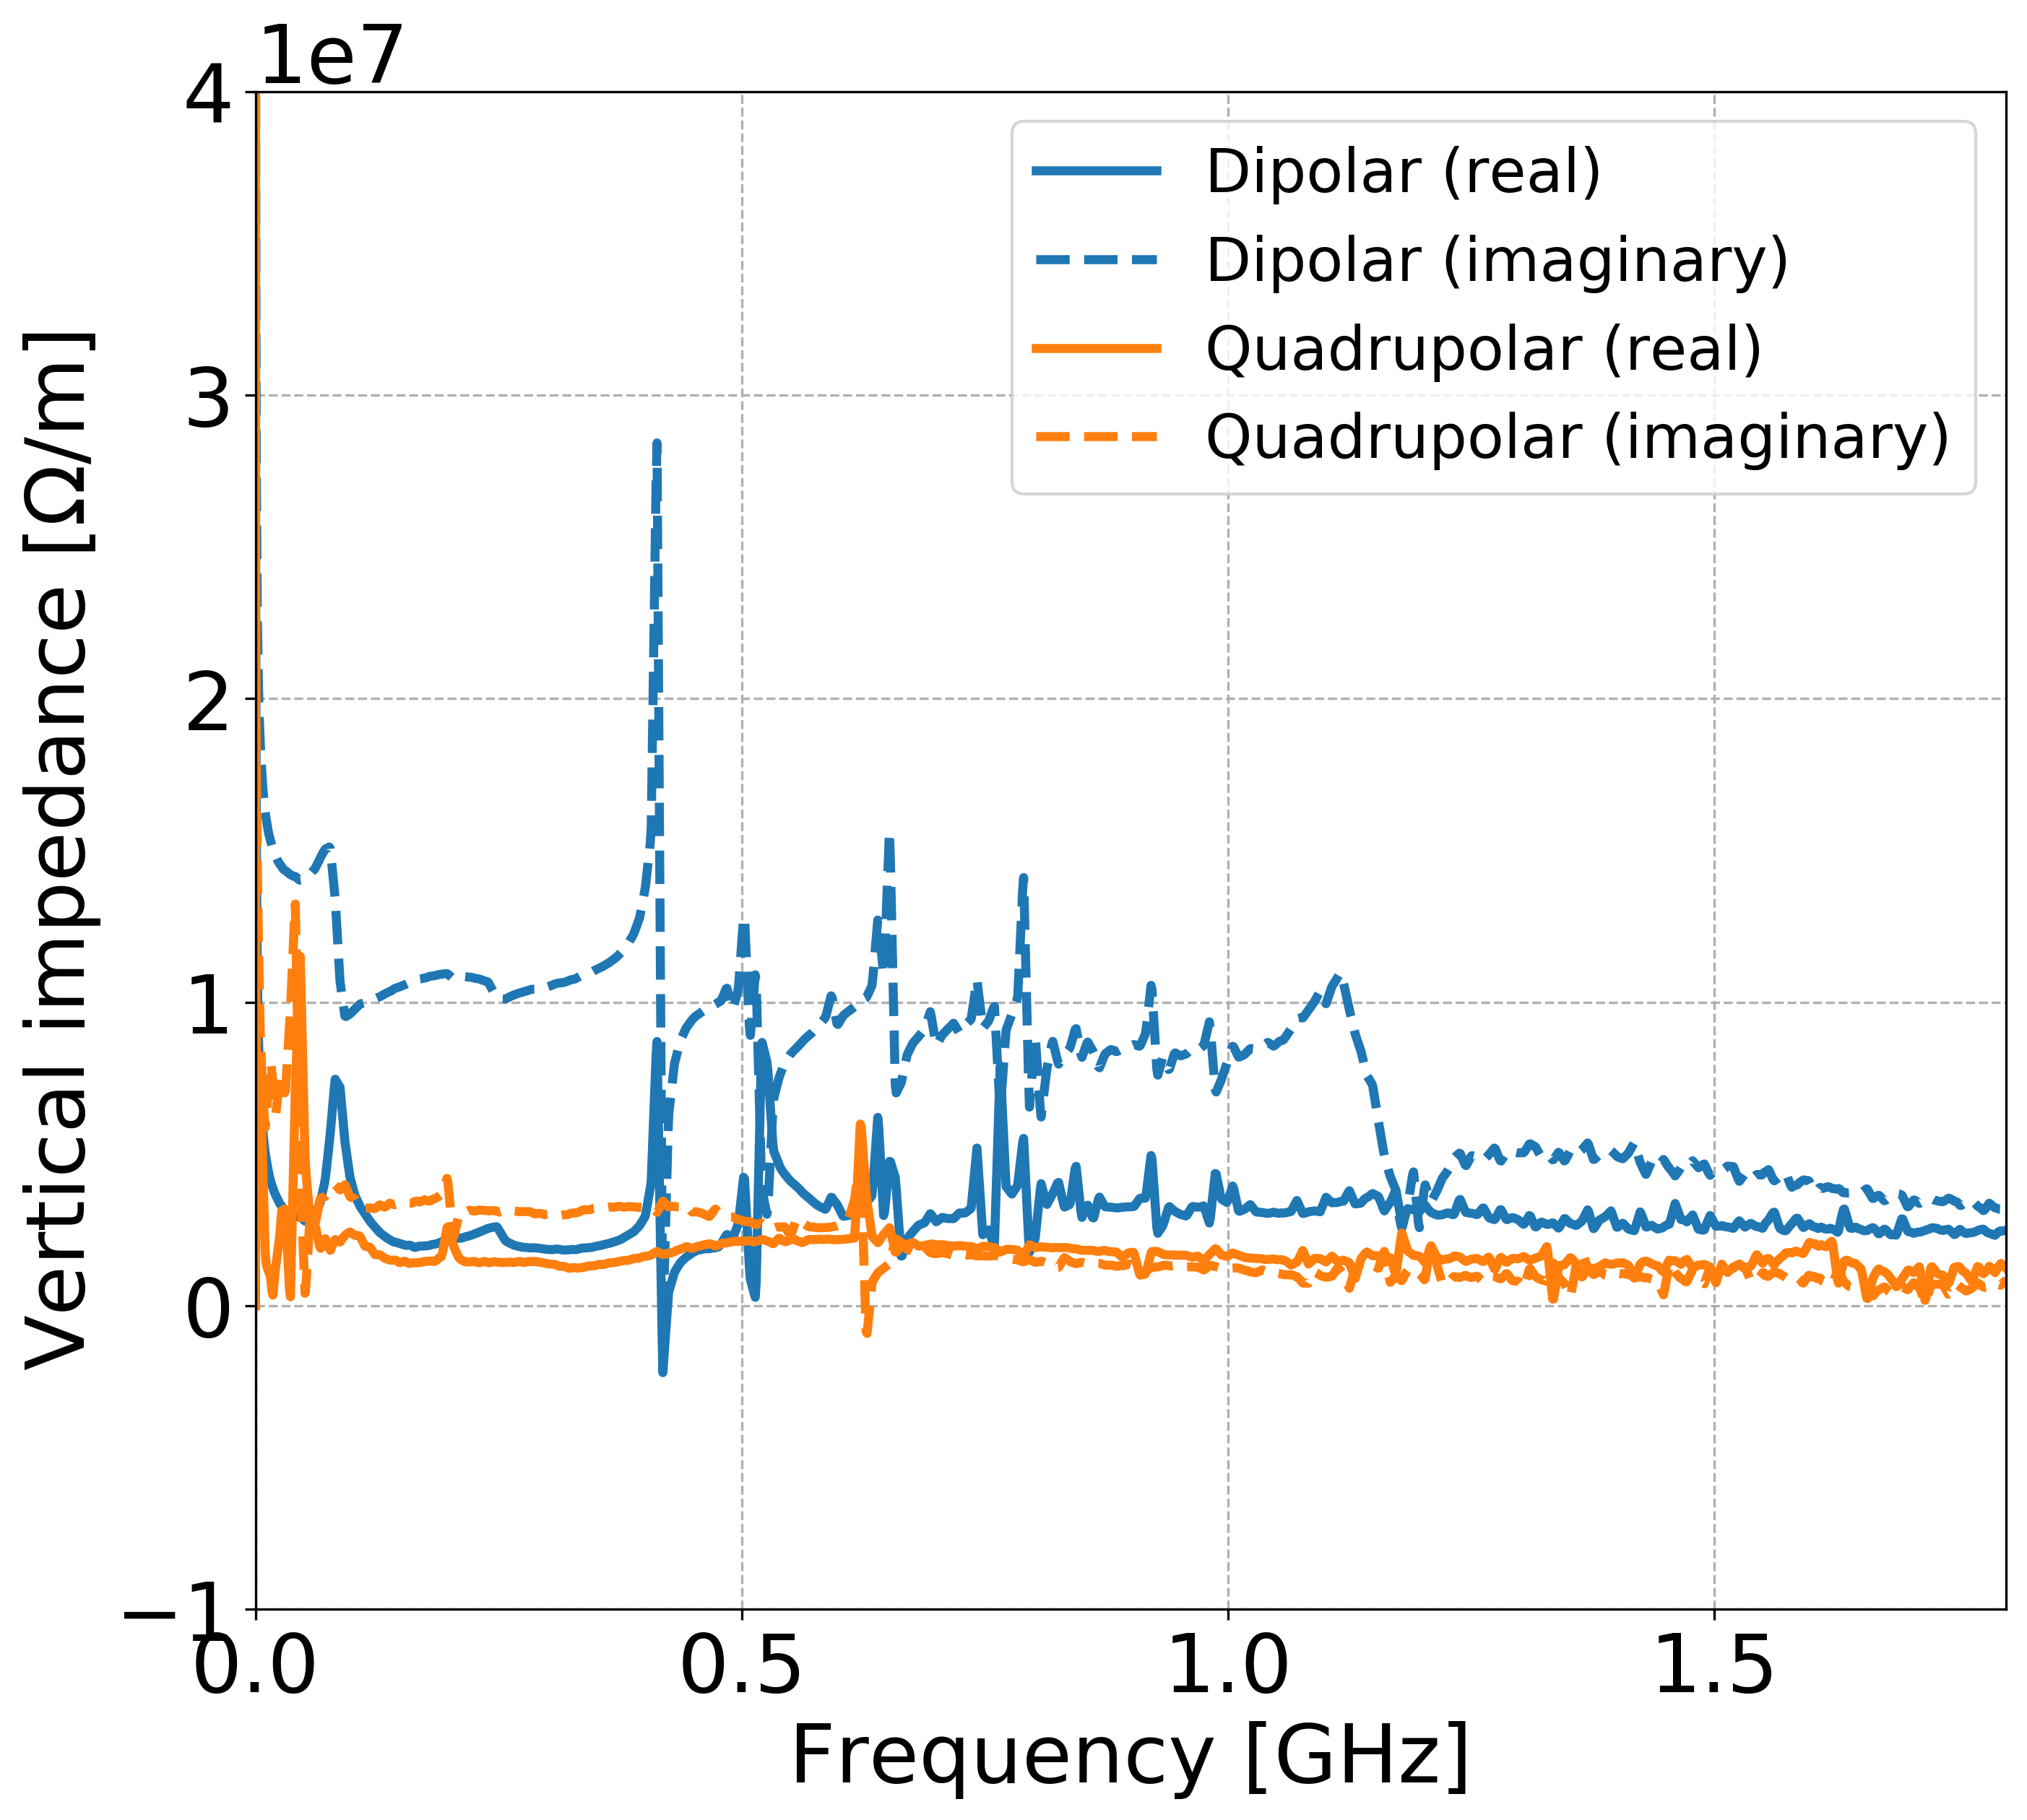
\includegraphics[width=1\textwidth]{images/Ch7/Q26_complete_SPS_model_impedance_V_plane.png}
        %\caption{Discrete Fourier transform}
        %\label{fig:add_label_here}
    \end{subfigure}
    \hfill
     \caption{Horizontal (left) and vertical (right) impedance model of the SPS. The model is available in the public gitlab repository of Ref.~\cite{sps_impedance_model_git}.} % bunch passage
     \label{fig:sps_impedance_model_H_V}
 \end{figure}

 The contributions from the wall, the kickers and the step transitions are visible at the low freqencies (up to $\sim$ 0.4\,GHz). The impedance of the RF cavities and the beam position monitors (BPMs) corresponds results to the peaks observed between $\sim$ 0.4-1\,GHz. 
%https://indico.cern.ch/event/299470/contributions/686509/attachments/564150/777102/LIUSPS_transverse_imp_5.pdf %For a clearer picture, it is worth mentioning that at low freqencies (up to $\sim$ 0.4\,GHz) the impedance is mainly from the wall the kickers and the step transitions. The peaks between $\sim$ 0.4-1\,GHz appear due to the RF cavities and the beam position monitors.
%https://indico.cern.ch/event/299470/contributions/686509/attachments/564150/777102/LIUSPS_transverse_imp_5.pdf

\normalsize{\textbf{Wake functions}}\\
As already discussed in Section~\ref{subsec:pyheadtail}, in order to include the impedance effects in PyHEADTAIL simulations the real-value wakefields in time domain are used. The wakefield kicks are computed as a convolution of the wake function with the moments of each particle. The total transverse dipolar (blue) and quadrupolar (orange) wake functions for both planes of the SPS can be found in the gitlab repository of Ref.~\cite{sps_impedance_model_git} and they are plotted in Fig~\ref{fig:sps_wakefunctions_model_H_V}.

% Plot figures: /eos/user/n/natriant/Project_thesis/plot_wakefields_impedances_SPS
 \begin{figure}[!ht]
    \centering
    \begin{subfigure}[t]{0.45\textwidth}
        \centering
        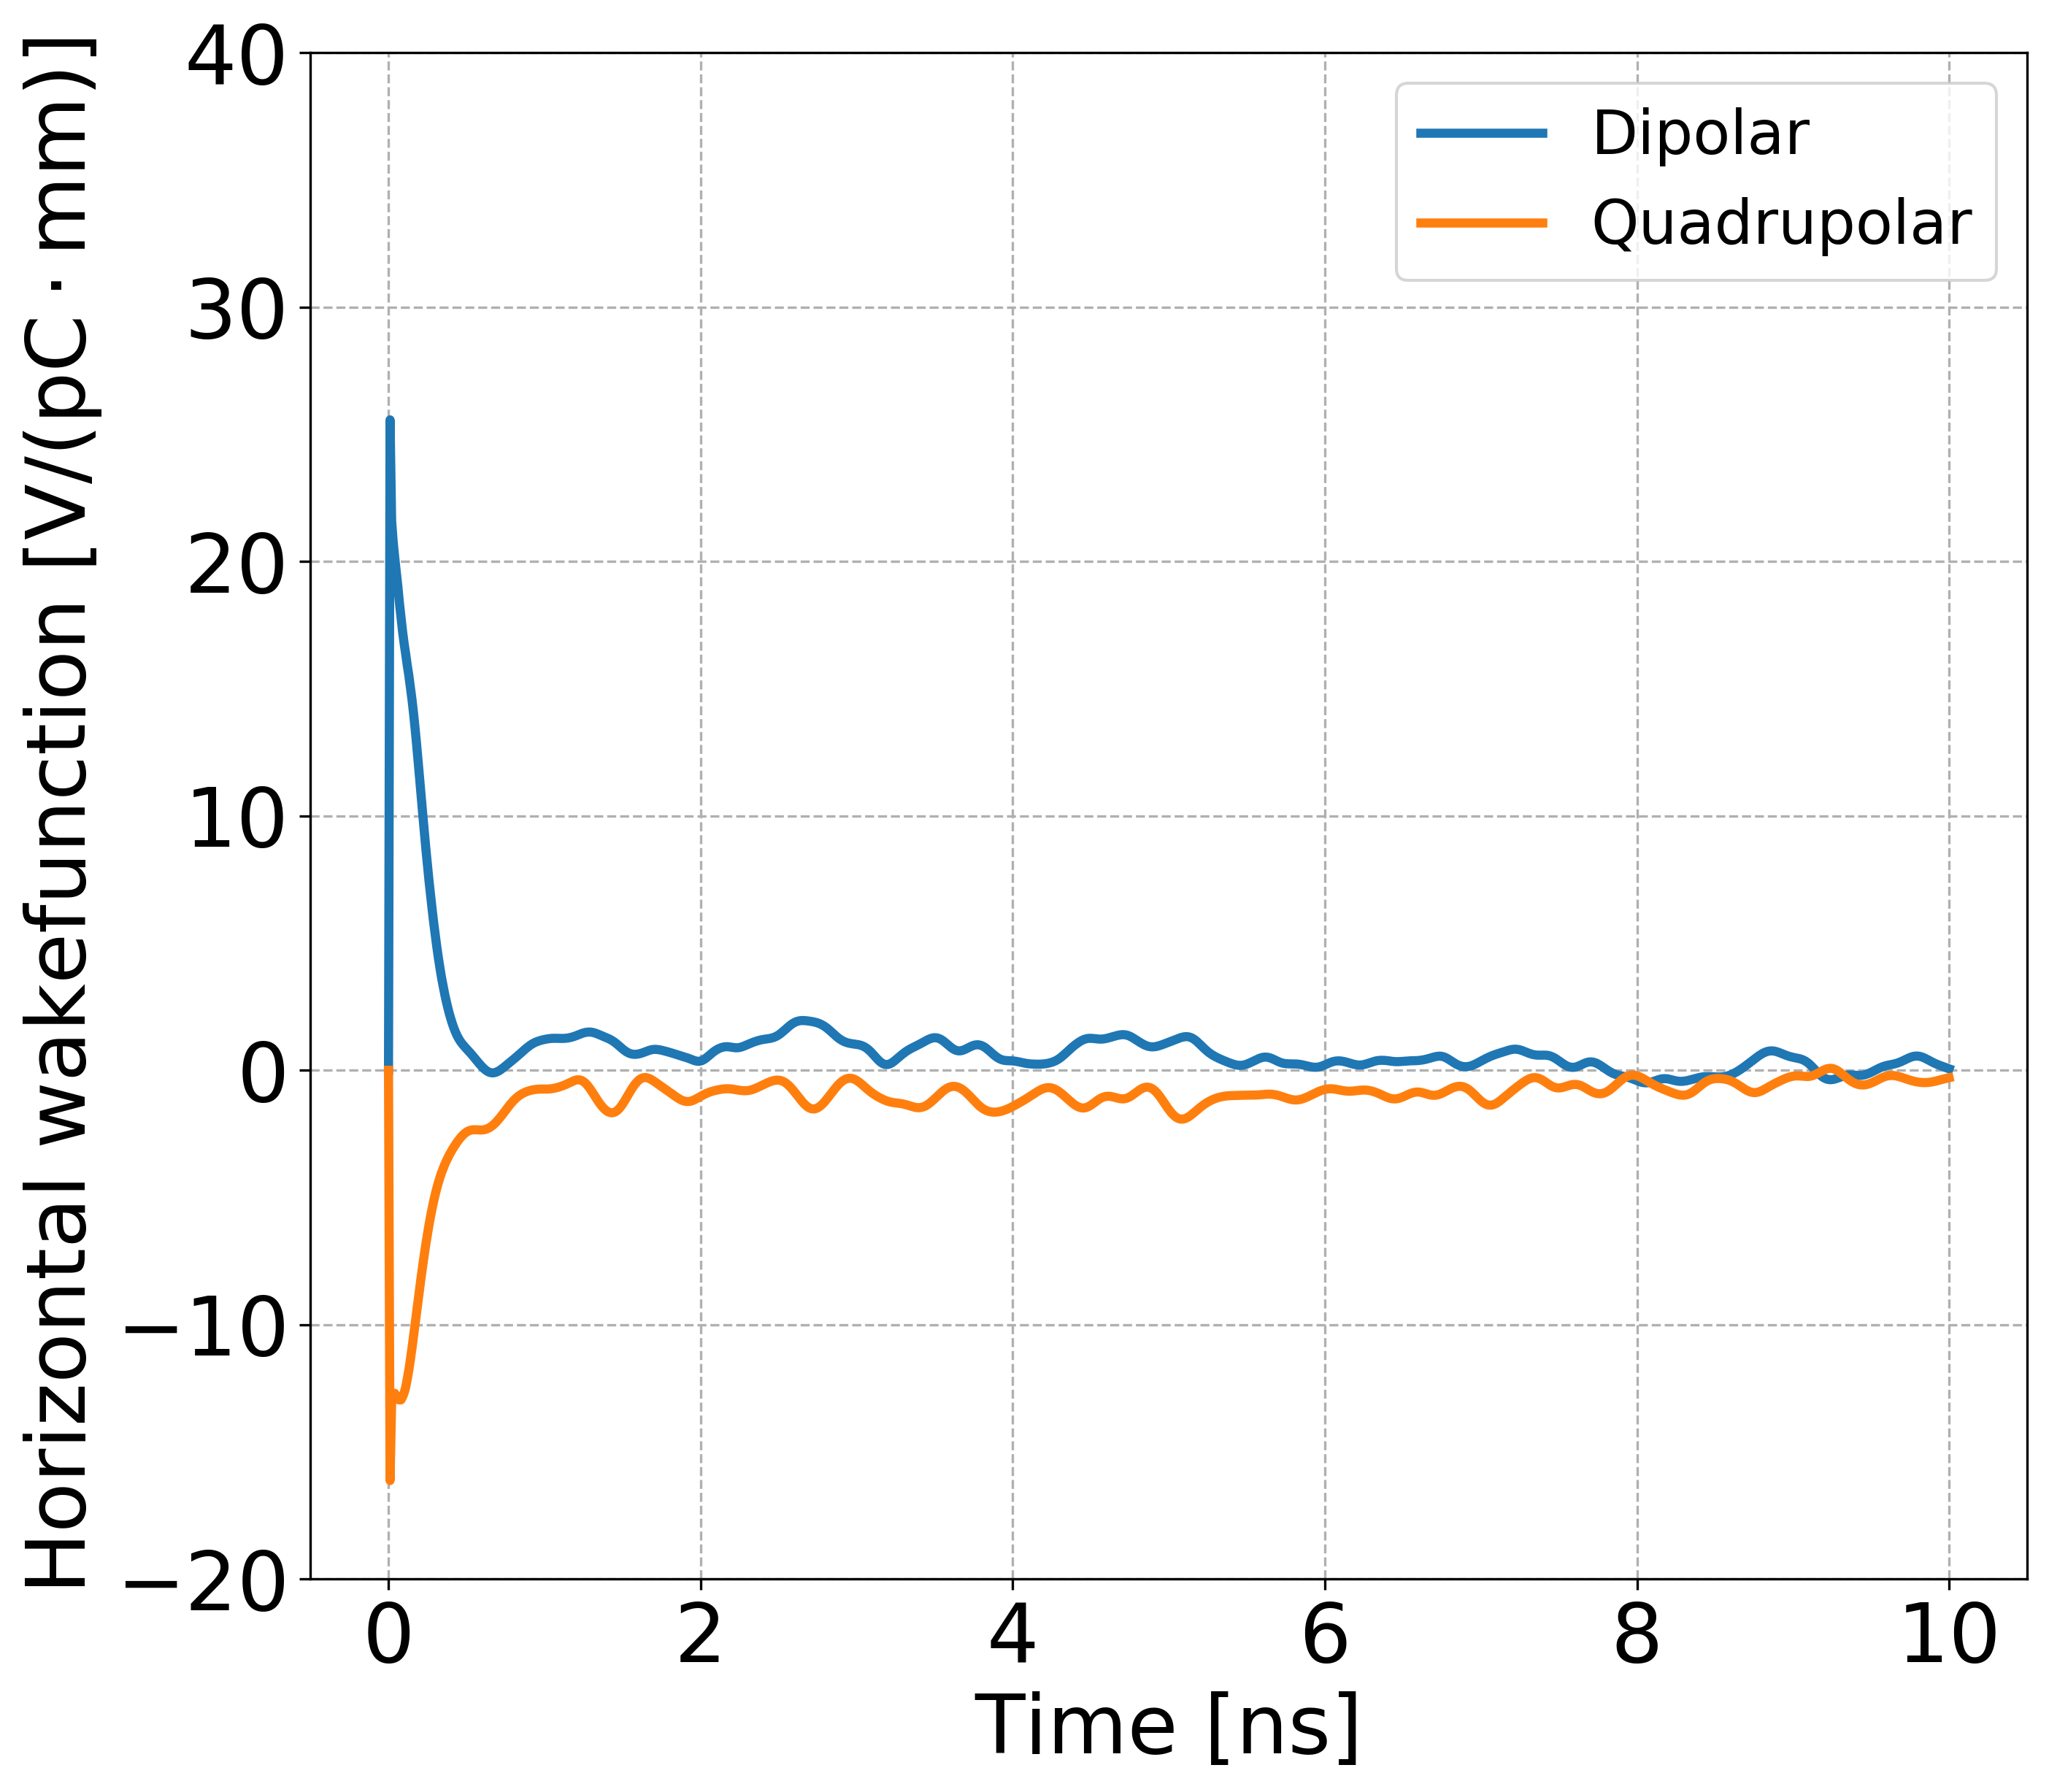
\includegraphics[width=1\textwidth]{images/Ch7/Q26_complete_SPS_model_wakefunctions_H_plane.png}
        %\caption{$y=\sin(2 \pi f t),\ f=50$ Hz}
        %\label{fig:add_label_here}
    \end{subfigure}
    \hfill
    \begin{subfigure}[t]{0.45\textwidth}
        \centering
        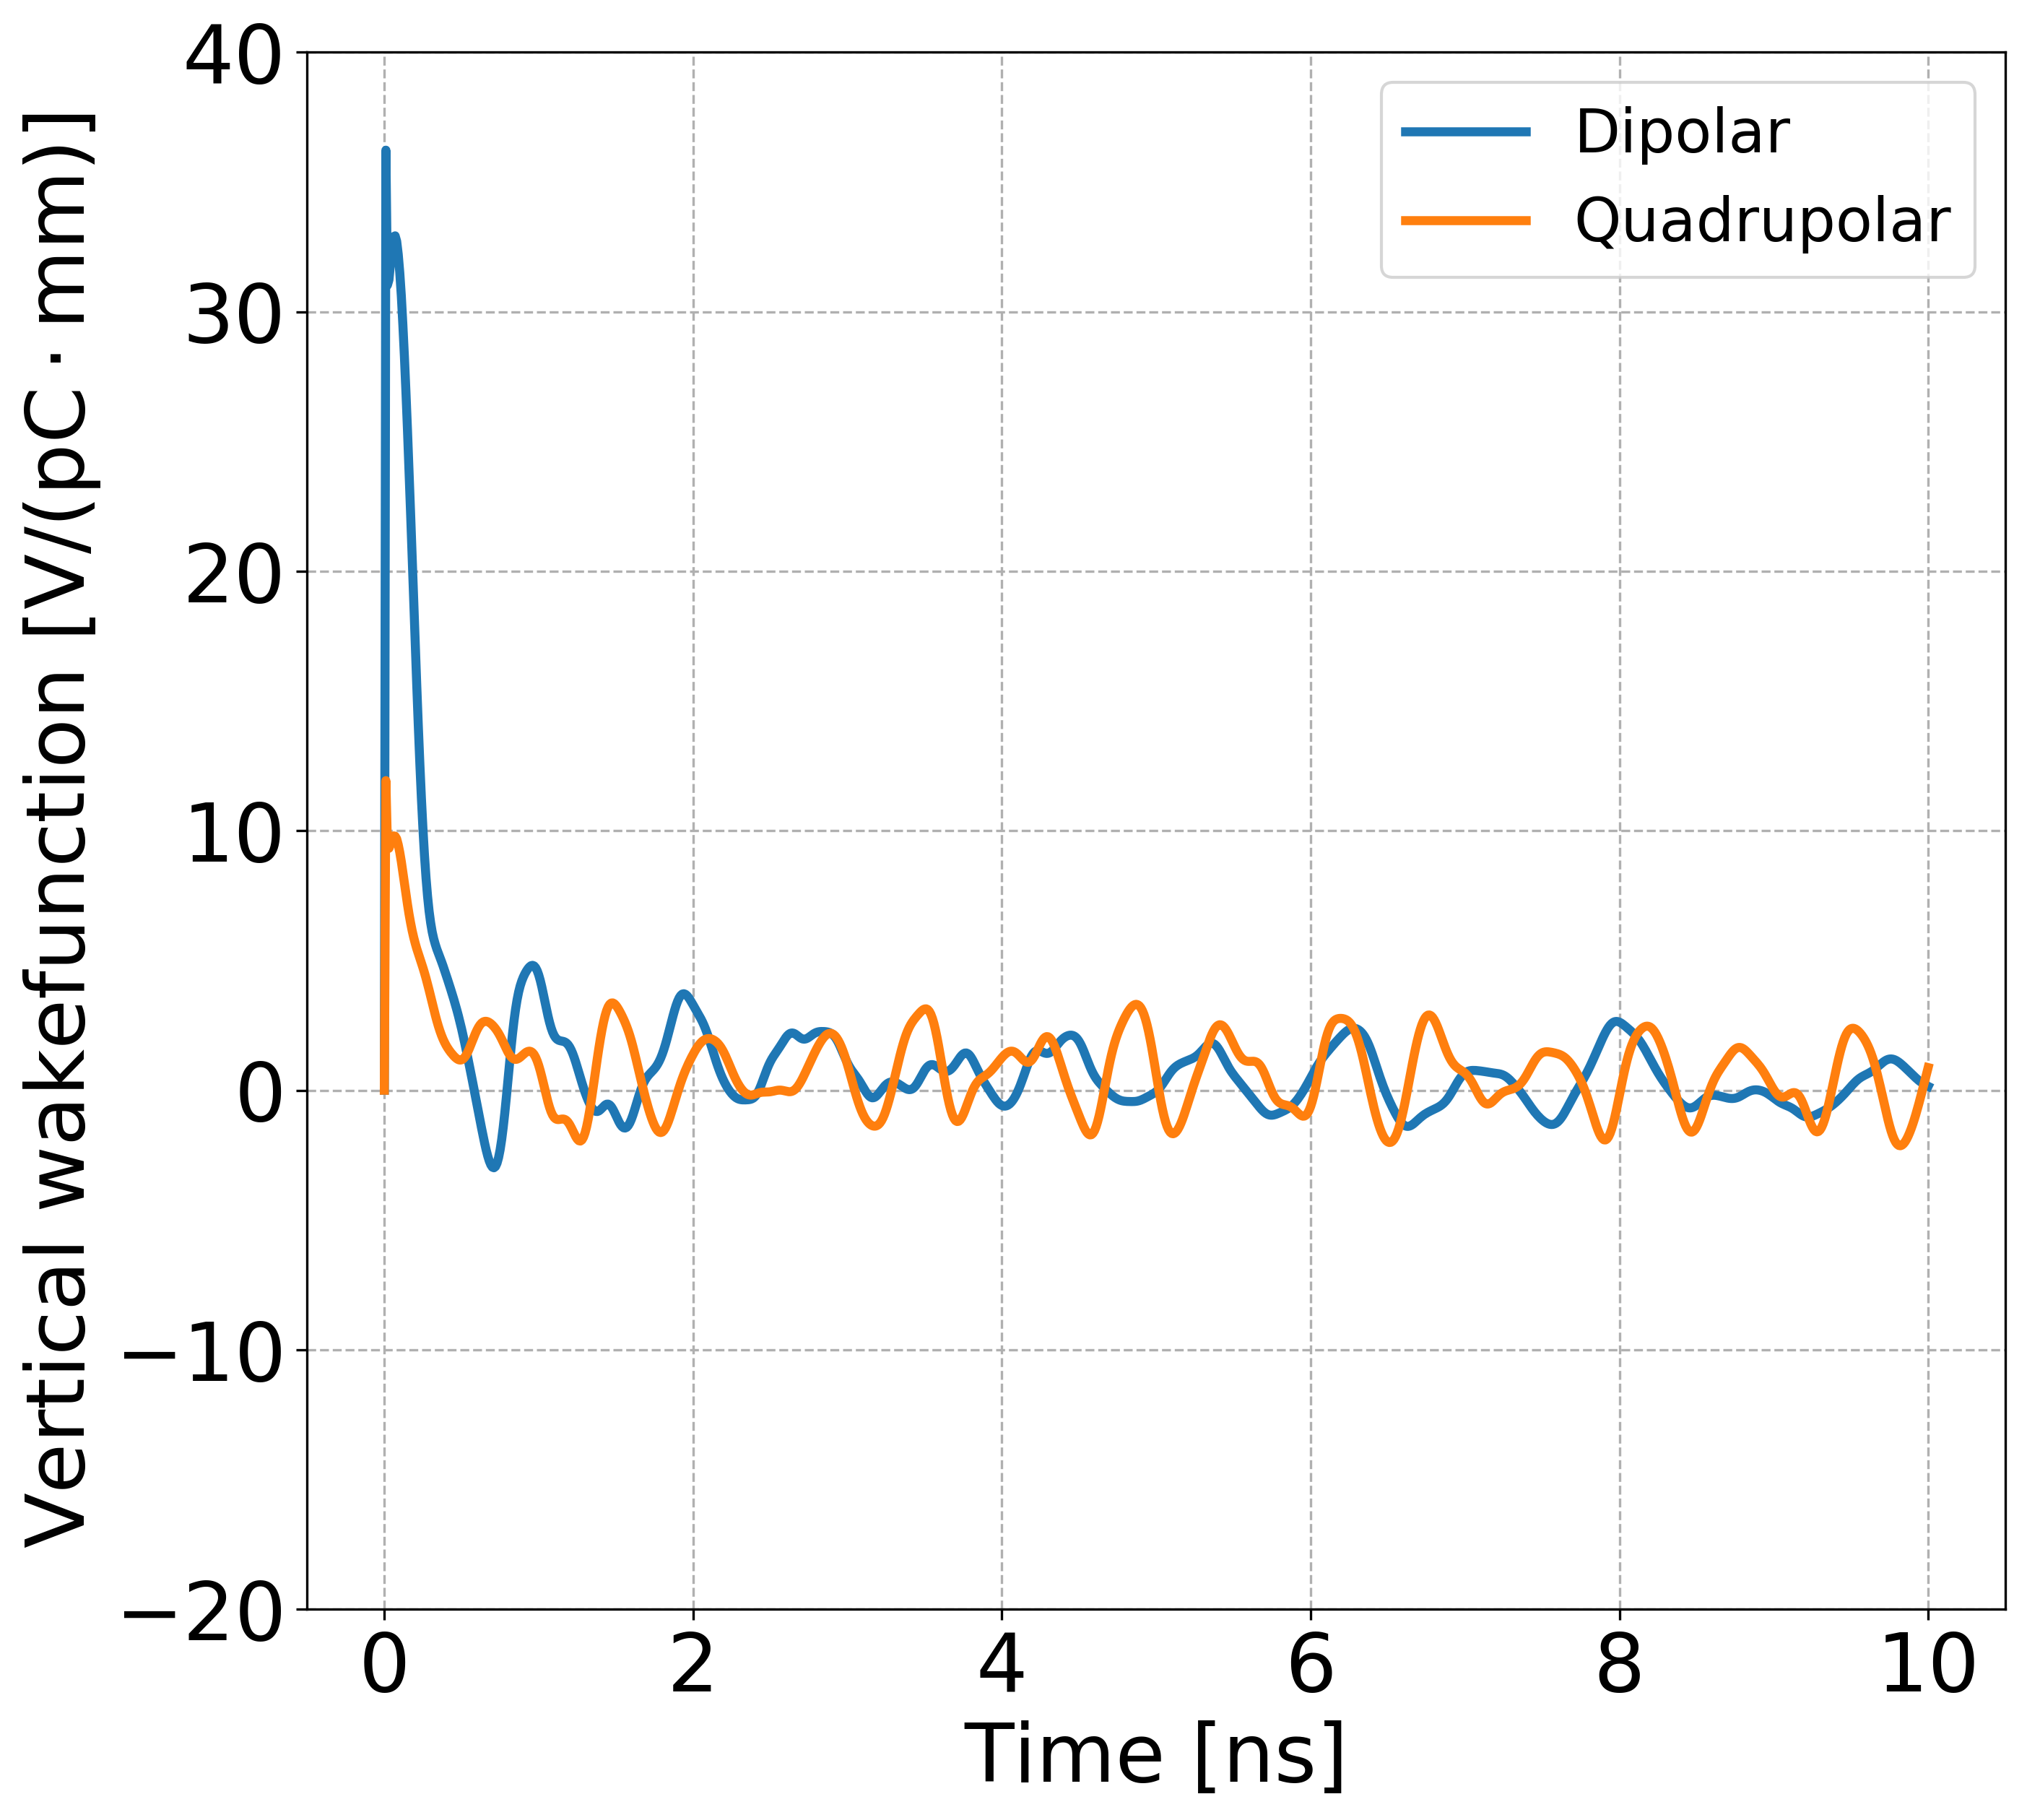
\includegraphics[width=1\textwidth]{images/Ch7/Q26_complete_SPS_model_wakefunctions_V_plane.png}
        %\caption{Discrete Fourier transform}
        %\label{fig:add_label_here}
    \end{subfigure}
    \hfill
     \caption{Horizontal (left) and vertical (right) wakefunctions of the SPS. The wake functions are available in the public gitlab repository of Ref.~\cite{sps_impedance_model_git}. For comparison the bunch length in the SPS CC experiments is $\sim$ 1.85\,ns (4$\mathrm{\sigma_t}$).} % bunch passage
     \label{fig:sps_wakefunctions_model_H_V}
 \end{figure}

It should be highlighted that the impedance model is not obtained from a simple Fast Fourier Transform algorithm on the wakefunctions but rather with more complex procedures described in the references provided above. Last the imepdance model is used as an input in the Sacherer formula (Eq.~\eqref{eq:complext_tune_shift_modes_m}) for analytical estimations while the wake functions are used as an input in simulation codes such as PyHEADTAIL.


% slide 9 https://accelconf.web.cern.ch/ipac2019/talks/weypls1_talk.pdf

% Carlo Zaninni thesis: s, it is important to have an accurate description of the wake at a distance z significantly smaller than the RMS bunch-length, which means that the impedance calculation needs to be accurate up to very high frequency (depending on the accelerator we consider, from a few GHz to the range of THz). 

\subsection{Testing the implementation in PyHEADTAIL}\label{subsec:test_implementation_pyheatail}
As discussed in Section~\ref{subsec:wakefields} the imaginary part of the impedance leads to a coherent tune shift which depends on the bunch intensity. One of the most common ways to test the correct implementation of the impedance model in a tracking simulation code is to benchmark the simulated intensity-dependent coherent tune shift with the theoretically predicted behavior (using Eqs.~\eqref{eq:complext_tune_shift_modes_m} and ~\eqref{eq:real_tunu_mode_l}).

Typically, in tracking simulations, the coherent tune is obtained by applying a frequency analysis technique to the oscillations of the centroid of the particle distribution (the center of mass of the bunch). Here, the analysis is limited to the coherent mode $l=0$ as it can be obtained using a simple Fast Fourier Transform (FFT) algorithm~\cite{FFT_and_applications}. Higher modes (in absolute value, i.e. $l=\pm 1, \pm 2$ etc) can be obtained with more complex algorithms such as the oned provided from the SUSSIX code~\cite{Bartolini:702438} \footnote{The SUSSIX code is applied to the complex position in phase space, $u-i p_u$, while an FFT algorithm is applied only to the transverse position $u$, where $u=(x,y)$~\cite{Salvant:1274254}.}. Nevertheless, the study of mode $l=0$ is sufficient for the purpose of the studies presented here. For simplicity in the following the term "coherent tune" will refer to the coherent tune of mode $l=0$.

\textbf{Simulations setup}\\
The parameters used for setting up the linear transfer map, the longitudinal tracking, and the beam initialisation are shown in Table~\ref{tab:pyheadtail_simulation_parameters} and are the ones used in the SPS $\CC$ experiment of 2018. The ring is consisted of one segment, with one interaction point at which the beam interacts with the wakefields. At that location, the horizontal and vertical beta functions equal the corresponding average beta functions over the SPS machine (see Section~\ref{subsec:pyheadtail}). The latest transverse wakefield model (as of February 2019 in Ref.~\cite{sps_impedance_model_git}) of the SPS was used.

The bunch poulation of the different intensity values, was represented by $5 \times 10^5$ macroparticles and the number of slices of the longitudinal distribution was 500.

\begin{table}[!hbt]
	\begin{minipage}{\textwidth}
      \begin{centering}
   \caption{PyHEADTAIL simulation parameters used to study impedance induced effects for the SPS.}
	\begin{tabu} to \textwidth {X[c,m] X[0.5c,m] X[0.5c,m] X[0.01c,m]}
		&&& \\[-6mm]
		\toprule \toprule
		\multicolumn{2}{l}{\textbf{Parameter}} &
		\multicolumn{2}{c}{\textbf{Value}} \\
		\bottomrule
      \multicolumn{2}{l}{Beam energy, $\symE$} & \multicolumn{2}{c}{270\,GeV} \\
      \multicolumn{2}{l}{Machine circumference, $C_0$}  & \multicolumn{2}{c}{6911.5623\,kHz} \\
      \multicolumn{2}{l}{Horizontal / Vertical betatron tune, $\Qx$ / $\Qy$}  & \multicolumn{2}{c}{26.13 / 26.18} \\
      \multicolumn{2}{l}{Synchrotron tune, $\Qs$}  & \multicolumn{2}{c}{0.0051}\\
      \multicolumn{2}{l}{Momentum compaction factor, $\alpha_p$}  & \multicolumn{2}{c}{1.9 $\times 10^{-3}$}\\
      \multicolumn{2}{l}{Number of bunches}  & \multicolumn{2}{c}{1} \\
      \multicolumn{2}{l}{Rms bunch length, 4$\sigmat$}  & \multicolumn{2}{c}{1.7\,ns}\\
      \multicolumn{2}{l}{Horizontal / Vertical normalised emittance, $\epsilon_x$ / $\epsilon_y$}  & \multicolumn{2}{c}{2\,$\mathrm{\mu m}$ / 2\,$\mathrm{\mu m}$}\\
      \multicolumn{2}{l}{Average horizontal / vertical beta function, $\langle \beta_x \rangle / \langle \beta_y \rangle$}  & \multicolumn{2}{c}{42.0941\,m / 42.0137\,m $^\ast$ } \\
      \bottomrule
      \multicolumn{2}{l}{Number of macroparticles, $N_\mathrm{mp}$}  & \multicolumn{2}{c}{$5 \times 10^5$} \\
      \multicolumn{2}{l}{Number of longitudinal slices, $N_\mathrm{slices}$}  & \multicolumn{2}{c}{500} \\
      \bottomrule
	\end{tabu}
   \label{tab:pyheadtail_simulation_parameters}
   \end{centering}\footnotesize{$^\ast$ Model values for the Q26 optics.}
   \end{minipage}
\end{table}

For all the PyHEADTAIL simulation studies presented in this thesis, the Twiss parameter $\alpha_u(s)$ and the dispersion function $D_u(s)$ equal zero. This is a valid assumption for the studies as these parameters have no direct impact on the effects under investigation.

To facilitate the observation of the coherent tune, the bunch was intialised with a static offset of 0.15$\sigma_{x,y}$ in both transverse planes\footnote{The rms transverse beam size at the only interaction point along the ring i.e. at the location where the beam interacts with the wakefields.}, such as it performs dipole oscillations around the machine. Then, it was tracked for 600 turns and the coherent tune was computed using a NAFF algorithm~\cite{LASKAR1990266, Kostoglou:2289645}, which provides a refined FFT analysis, and its python implementation, NAFFlib, can be found in the corresponding package in Ref.~\cite{nafflib_repository}, on the turn-by-turn centroid motion. The coherent tune shift was computed by subtracting the obtained tune value from the unperturbed coherent tune (in the absence of impedance) which equals the $Q_{u0}$ value.


Finally, the dependence of the coherent tune on the intensity value was studied in the absence of other detuning effects (such as chromaticity or detuning with transverse amplitude, even though they mainly introduce incoherent tune shifts). % Do they also introduce some small coherent tune?

The simulation was repeated for a range of bunch intensities, $N_b$, equally-spaced from 0 to $5 \times 10^{10}$ protons per bunch. This range was chosen to be in the vicinity of the bunch intensity of the $\CC$ experiments of 2018, where $N_b$ was $3\times 10^{10}$ protons per bunch. $N_b=0$ is not a realistic value. However, it is used here as the reference point for which the coherent betatron tune equals zero. The simulation results are plotted against the theoretically expected tune shifts in Fig.~\ref{fig:sps_coherent_DQ_vs_intensity_original_complete_model}.

The theoretically expected values are computed from Eqs.~\eqref{eq:complext_tune_shift_modes_m} and ~\eqref{eq:real_tunu_mode_l} for $l=0$ and using only the imaginary part of the imepdance. Given that $\Gamma(1/2)=\sqrt{\pi}$ and $Q_u = \omega_{u0}/\omega_\mathrm{rev}$ equation Eq.~\eqref{eq:complext_tune_shift_modes_m} becomes:
\begin{equation}\label{eq:real_tune_shfit_for_coherent_mode}
    \Delta \Omega_u^{(0)} =  \Omega_{u0}^{(0)} - \omega_{u0} = \frac{\sqrt{\pi}}{4 \pi}\frac{N r_0 c^2}{\gamma_0 \frac{2\pi}{\omega_\mathrm{rev}}\omega_u \sigma_z} Z_\mathrm{eff, im} = \frac{N r_0 c^2}{8 \pi^{3/2} \gamma_0 Q_u \sigma z}Z_\mathrm{eff, im}
\end{equation}
All the parameters inserted in Eq.~\eqref{eq:real_tune_shfit_for_coherent_mode} should be converted in CGS (centimetre–gram–second) units.

Then the coherent betatron tune shift is computed by inserting the result of Eq.~\eqref{eq:real_tune_shfit_for_coherent_mode} in Eq.~\eqref{eq:real_tunu_mode_l} such as 
\begin{equation}
    \Delta Q_u = \frac{\Delta \Omega_u^{(0)}}{\omega_\mathrm{rev}}.
\end{equation}


 % pyheadtail_data/final_for_thesis/2018_conditions/study_0_DQ_vs_intensity/
\begin{figure}[!ht]
    \centering
    \begin{subfigure}[t]{0.45\textwidth}
        \centering
        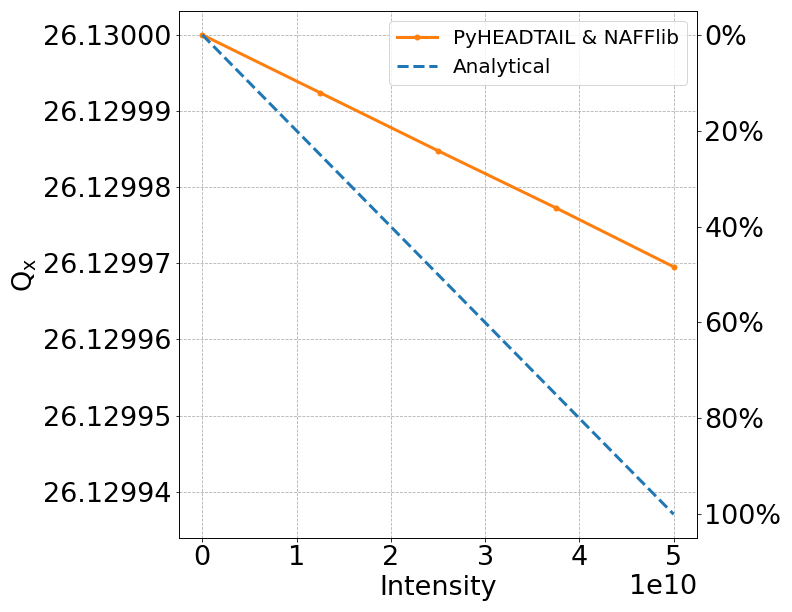
\includegraphics[width=1\textwidth]{images/Ch7/Qx_vs_intensity_complete_impedance_sps_q26model_MD2018_parameters.png}
        %\caption{$y=\sin(2 \pi f t),\ f=50$ Hz}
        %\label{fig:add_label_here}
    \end{subfigure}
    \hfill
    \begin{subfigure}[t]{0.45\textwidth}
        \centering
        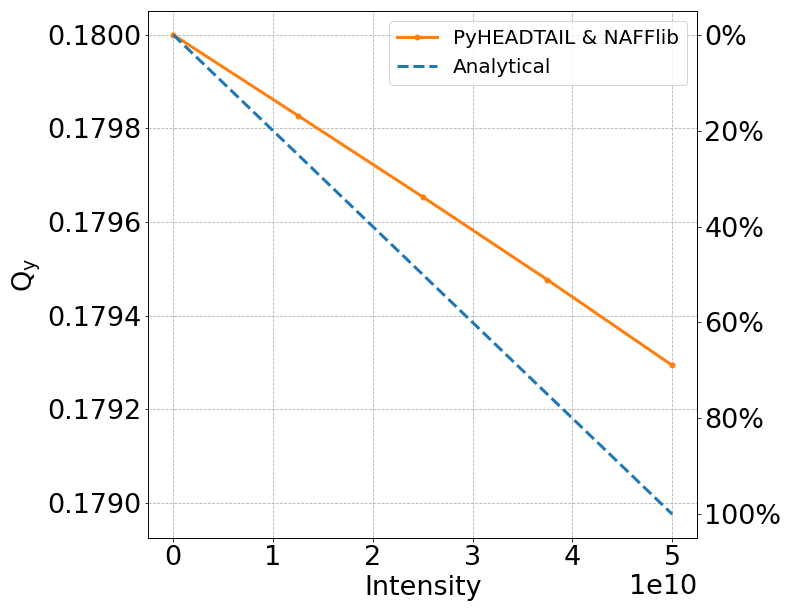
\includegraphics[width=1\textwidth]{images/Ch7/Qy_vs_intensity_complete_impedance_sps_q26model_MD2018_parameters.png}
        %\caption{Discrete Fourier transform}
        %\label{fig:add_label_here}
    \end{subfigure}
    \hfill
     \caption{Horizontal (left) and vertical (right) coherent tunes as a function of intensity in the presence of the beam coupling SPS imepdance obtained using analytical formula (blue dashed line) and PyHEADTAIL tracking simulations (orange line). The impedance model and the wake functions used are available in the public gitlab repository of Ref.~\cite{sps_impedance_model_git}.} % bunch passage
     \label{fig:sps_coherent_DQ_vs_intensity_original_complete_model}
 \end{figure}

 Figure~\ref{fig:sps_coherent_DQ_vs_intensity_original_complete_model} shows that the coherent tune shift from the analytical model does not agree with simulation results. In particular the wakefields implementation in the PyHEADTAIL results just to $\sim 50 \%$ and $\sim 70 \%$ of the total coherent tune shift estimated using the analytical formula of Sacherer with the impedance model. This discrepancy hadn't been observed before as this study has not been conducted for such low intensities (the usual intensity range for this type of study is in the order of $10^{11}$ protons per bunch ~\cite{Beck:2683038}) and short bunches. %p.101
 The analytical predictions from Sacherer formula have been repeatedly successfully benchmarked against beam measurements~\cite{Bartosik:1742183, sps_impedance_measurements_vs_model} which indicates that there is an issue with the model of the wakes or with their implementation in the simualtion. Given the fact that the studies with $\CC$s are quite sensitive on the coherent tune shift with intensity from the coupling impedance (this will be discussed in the following paragraphs of this chapter) it is crucial to identify the reason for the observed discrepancy and resolve it.

 After several studies and discussions with the experts on the topic \footnote{In particular with Carlo Zannini, carlo.zannini@cern.ch.} it was identified that the components of the resistive wall, the kickers, and the step transitions needed to be re-computed to provide higher accuracy at the lower frequencies. The details of this work are not discussed here as they are out of the scope of this thesis and they were not performed by the author. The re-computed wake functions along with the rest of the components of the original model can be found in the gihub repository of Ref. . and it will be reffered to as the "updated wakefields" model.

 The coherent betatron tune as a function of intensity obtained using PyHEADTAIL and the updated wakefields model is plotted in Fig.~\ref{fig:sps_coherent_DQ_vs_intensity_updated_model} against the analytical predictions from Sacherer formula. In the both transverse planes, the results from the simulations and the theory are in very good agreement ($\leq 5\%$) which is within the uncertainty that one can expect from the model implementation. 

 % pyheadtail_data/final_for_thesis/2018_conditions/study_0_DQ_vs_intensity/
\begin{figure}[!ht]
    \centering
    \begin{subfigure}[t]{0.45\textwidth}
        \centering
        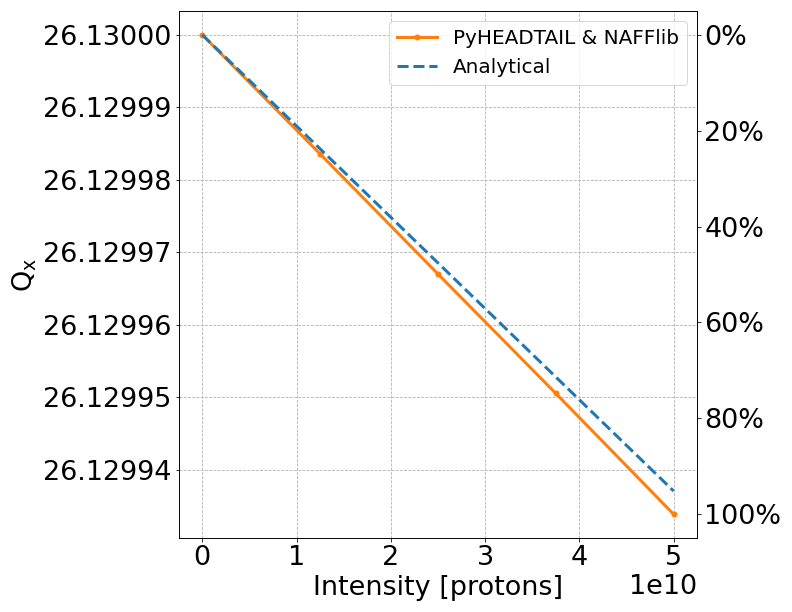
\includegraphics[width=1\textwidth]{images/Ch7/Qx_vs_intensity_complete_impedance_sps_q26model_updated_MD2018_parameters_integer.png}
        %\caption{$y=\sin(2 \pi f t),\ f=50$ Hz}
        %\label{fig:add_label_here}
    \end{subfigure}
    \hfill
    \begin{subfigure}[t]{0.45\textwidth}
        \centering
        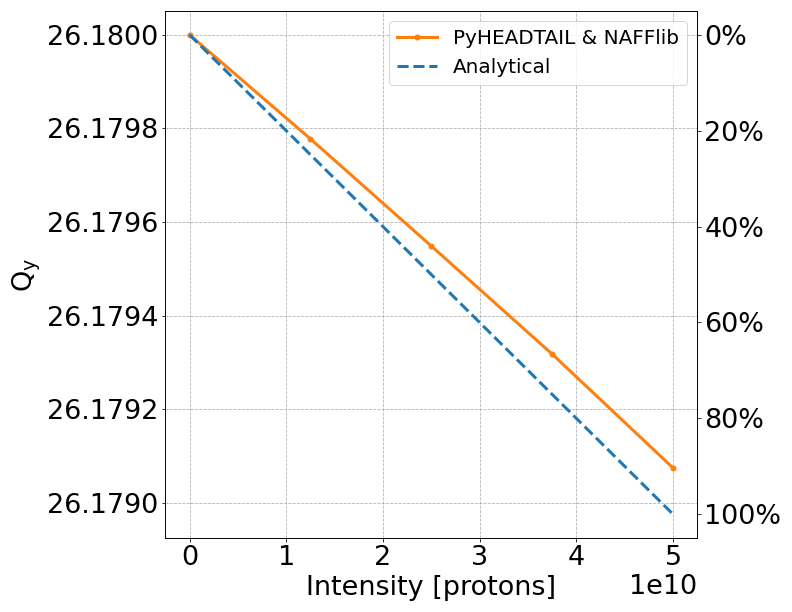
\includegraphics[width=1\textwidth]{images/Ch7/Qy_vs_intensity_complete_impedance_sps_q26model_updated_MD2018_parameters_integer.png}
        %\caption{Discrete Fourier transform}
        %\label{fig:add_label_here}
    \end{subfigure}
    \hfill
     \caption{Horizontal (left) and vertical (right) coherent tunes as a function of intensity in the presence of the beam coupling SPS imepdance obtained using analytical formula (blue dashed line) and PyHEADTAIL tracking simulations (orange line). The impedance model and the wake functions ("updated wakefields" model) used are available in the public repositories of Ref.~\cite{sps_impedance_model_git} and Ref.. respectively.} % bunch passage
     \label{fig:sps_coherent_DQ_vs_intensity_updated_model}
 \end{figure}

 The above figure confirms the correct implementation of the updated wakefields model in PyHEADTAIL and therefore it will be used to study the interplay of the $\CC$ noise induced emittance growth with impedance induced effects. These studies are presented in the following chapter.

\section{Emittance growth simulations setup}\label{sec:setup_simulations_emit_growth}
The simualtions that were performed to investigate the impact of the beam coupling impedance on the $\CC$ RF noise-induced emittance growth were performed following the procedure and using the parameters that are described below. Any change in the choice of parameters, e.g. for some of the parametric studies, will be mentioned in the corresponding paragraph.

The parameters used for setting up the linear transfer map, the longitudinal tracking, and the beam initialisation are shown in Table~\ref{tab:pyheadtail_simulation_parameters} and are the ones used in the SPS $\CC$ experiment of 2018. The ring is consisted of two segments with two interaction points. In the first one $\CC$ noise-like kicks are applied on the beam particles while in the second one the the beam interacts with the wakefields as discussed in the previous section. The updated wakefields model Ref... of the SPS was used.

At the location of the $\CC$ RF noise kick the horizontal and vertical beta functions equals the values at the location of the $\CC2$ which was used in the experiments of 2018. At the location, where the wakefield kicks are applied the transverse beta functions equal the corresponding average beta functions over the SPS machine (see Section~\ref{subsec:pyheadtail}). 

As already discussed in the previous section, the simualtions are performed for the Twiss parameter $\alpha_u(s)$ and the dispersion function $D_u(s)$ equal zero. This is a valid assumption for the studies as these parameters have no direct impact on the effects under investigation.

The emittance growth studies were performed for intensity of $3 \times 10^{10}$ protons per bunch and for linear chromaticity of $Q^{\prime}_{x,y}=0.5$ in accordance with the 2018 experiments. The bunch population was represented by $5 \times 10^{5}$ macroparticles and the number of longitudinal slices was 500. The emittance growth was also simulated without including the wakefields. For that case the bunch population was represented by $10^{5}$ particles and no longitudinal slicing was applied.

At the location of the $\CC$ RF noise kick, the angle, $y^\prime$, of each particle within the bunch is updated every turn according to the kicks of Eqs.~\eqref{eq:amplitude_noise_kick} and ~\eqref{eq:phase_noise_kick} for amplitude and phase noise kick respectively. The noise level is stronger than the ones of the actual $\CC$ RF system and was chosen such as it results in a reasonable growth in the simulation time of $10^5$ turns (it corresponds to $\sim$ 2.5 seconds in the SPS). This approach is valid due to the linear growth of emittance with time and the linear scaling with the noise level~\cite{PhysRevSTAB.18.101001}. The parameters used for the implementation of the $\CC$ RF noise kick in the simulations are shown in Table~\ref{tab:CC_pyheadtail_simulation_parameters}.

\begin{table}[!hbt]
	\begin{minipage}{\textwidth}
      \begin{centering}
   \caption{PyHEADTAIL simulation parameters used for the implementation of the CC RF noise kicks for the emittance growth studies. This table is complementary of Table~\ref{tab:CC_pyheadtail_simulation_parameters}.}
	\begin{tabu} to \textwidth {X[c,m] X[0.5c,m] X[0.5c,m] X[0.01c,m]}
		&&& \\[-6mm]
		\toprule \toprule
		\multicolumn{2}{l}{\textbf{Parameter}} &
		\multicolumn{2}{c}{\textbf{Value}} \\
		\bottomrule
      \multicolumn{2}{l}{Horizontal / vertical beta function, $\beta_{x, \mathrm{CC}} / \beta_{y, \mathrm{CC}}$}  & \multicolumn{2}{c}{30.31\,m / 73.82\,m } \\
      \multicolumn{2}{l}{CC frequency, $f_\mathrm{CC}$}  & \multicolumn{2}{c}{400.78\,MHz} \\
      \multicolumn{2}{l}{Scaling factor for amplitude and phase noise, $A$}  & \multicolumn{2}{c}{$10^{-8}$} \\
      \bottomrule
	\end{tabu}
   \label{tab:CC_pyheadtail_simulation_parameters}
   \end{centering}
   \end{minipage}
\end{table}

As mentioned in Chapter~\ref{Ch:2018_analyisis} the Landau octupoles were switched off during the 2018 $\CC$ experiment. Nevetherless, a residual non-linearity was present in the machine mainly due to multipole components in the dipole magnets~\cite{Carlà:2664976, Alekou:2640326}. As the machine non-linearities were not explicitly characterised during the experiment, the dependence on the octupole-like amplitude dependent tune spread was studied. Instead of using an actual octupolar (non-linear) element which would result to resonance excitation\footnote{In the real SPS machine the Landau octupoles are installed in families of focusing and defocusing in order to avoid the excitation of resonances}, the amplitude dependent tune shift was introduced as changes to the phase advance of the particles depending on their individual action as discussed in Eq.~\eqref{eq:change_phase_advance_detunign}. More specifically, the dependence on the detuning coefficient in the vertical plane, $\alpha_{yy}$, was studied. For the studies presented in the following sections of this chapter, the horizontal detuning coefficient and the cross-term were left at zero for simplicity, i.e.~$\alpha_{xx} = \alpha_{xy} = 0$. % for better control over the simulations. This choice is also based on the fact that their value doesn't affect the results.
The sensitivity on the cross-term is discussed in the Chapter~\ref{Ch:experimental_CC_2022}, again for $\alpha_{xy} = 0$ as the horizontal coefficient does not affect the vertical emittance growth since there is no coupling between the two transverse planes.

The simulations were performed using an initial Gaussian bunch distribution in the six-dimensional phase space. This is a good approximation for the bunches used in the experimental studies of 2018. 

The geometric emittance value was computed every 100 turns (for computational efficiency) using the statistical definition which can be found in Eq.~\eqref{eq:geometric_emittance_v2}. The emittance growth rate was computed by performing a linear fit to the normalised (using Eq.~\eqref{eq:normalised_emittance}) emittance values over the simualtion turns ($N_\mathrm{turns}=10^5$). Twenty simulation runs were conducted, to reduce the uncertainty of the results. The initial distribution and the sequence of noise kicks was regenerated randomly every run. 





the sequence of noise
kicks was regenerated randomly for 20 run




Twenty simulation runs were conducted, to reduce the uncertainty of the results, for a white phase noise with power spectral density of $1.68 \cdot 10^{-10} \mathrm{rad^2/Hz}$. The noise power is much higher than in reality to get significant emittance growth during the course of the simulation. The emittance growth over the course of the simulation is comparable to that during a coast though. 





\section{First observations of emittance growth suppression by the impedance}

Show plot with the emittance evolution from the diffrent runs, in order to show that there is this spread, which is what corresponds to the error bar in the summary plots.


The effect of chromaticity is not taken into account in the computation of the tune spread, as it depends on the preriodic synchrotron motion and thus it cancells out.

\section{Characterisation of the emittance growth suppression by the impedance}

\section{Suppresion mechanism}\label{sec:suppression_mechanism}
\subsection{Past studies with beam-beam interactions}\label{subsec:past_studies_impedance_suppression_BB}
\subsection{Intensity scans}
\subsection{Schottky noise spectra}
